\section{Test} \label{sec:test}
Given that the aim of the project is to create a good code-base on which multiplayer games can easily be implemented, it is desirable that the server is stable and able to handle a large number of concurrent games without significant response time. More specifically we want a single server to be able to host as many games as possible without surpassing an average response time of 0.5 seconds. This time limit was chosen based on guidelines from Jakob Nielsen's ''Usability Engineering´´.\cite{response-time} The book states one second is the limit for which a user does not feel interrupted in using an application. We have then decided to be more strict, not wanting to get near this limit - This is why the target is 0.5 seconds.

Additionally we want to locate possible bottlenecks in the code, by recording the run time of each API call. This can be tested using black-box testing.

The tests were written as Python scripts, and can be found in the folder named Test with the rest of the source code. The raw test results can also be found inside this folder.

\subsection{Test Setup} \label{sec:testSetup}
The test is done by simulating active users through two scripts: one for simulating a number of active games, with the purpose of creating some artificial server load, and one for making single requests and collecting data.

The script designed to create server load, does so by requesting a thread on the server per desired game. Each thread creates an instance of a game, sends requests for game actions for the duration of the test and finally closes the game. Each thread ends up simulating very busy games with two requests per second.

The other script makes a single request 1000 times, collects the response delay for each request and finally calculates the mean and standard deviation.

Each script is run from separate computers, to be sure a bottleneck does not occur on the simulated client-side.

The server used was a HP Compaq 8200 Elite MT PC with the following setup.

\begin{itemize}
\item 64 bit Windows 7 Enterprise (Build 7601)
\item Intel Core i7-2600
\item 8 GB DDR3 RAM
\end{itemize}

\subsection{Analysis of Test Results}
After running the script the first time, a timeout exception was eventually thrown. We then modified the test to record these timeouts and continue the test, but the exact source of the exception was not located. On every iteration of the script that logs response times, the following requests were sent to the server.

\begin{itemize}
\item Login
\item Create game
\item Delete game
\item Join game
\item Leave game
\item Change location
\item Invite player
\item List public games
\item List joined games
\item Get game info
\item Shoot
\end{itemize}

The script was iterated 1000 times, and the requests that timed out were not included in the analysis of the final test results.

% % % tables
\Cref{tab:unloadgraph} shows the mean of response times for each request, when the server is not stressed. As seen in the table, the means are similar and well under 0.5 seconds for all requests, except for the \textit{Get joined games} call. We suspect this is because of the way data is stored in the database. This response time could be lessened by routinely deleting old games from the table containing created games.

The table also shows the number of requests exceeding the maximum allowed response time of 0.5 seconds. Again, \textit{Get joined games} is with 10 failures the most unreliable entry, but for all other requests only 1-3 out of the thousand calls exceeded the limit. Looking at the raw data, it can be seen the requests sometimes had a 4-6 second delay, and in rare cases completely timed out. It is difficult to pinpoint where the problem arises, but due to the low amount of slow or timed out requests, we argue that these results are satisfactory in regards to the delay threshold of 0.5 seconds.

\Cref{tab:loadgraph} shows the results of the test when the server was handling 100 busy games concurrently. By trial and error this was found to be the maximum amount of games the server could consistently handle without timing out completely, resulting in no requests returning.

The mean response for each request has increased from the response times in \Cref{tab:unloadgraph}. This is attributed to the increased load on the server from the 100 busy games running concurrently. \Cref{tab:loadgraph} also shows the \textit{Get joined games} request as having the worst mean response time, getting very close to the 0.5 second limit.

Not unexpectedly, it can be seen that there are more requests which exceed the delay threshold of 0.5 seconds. There are however less timeouts, indicating that the issue could be external to the server, for example a network issue.

% % % graph
Looking at the graph in \Cref{fig:loadgraph}, a general pattern can be seen. For the first approximately 90 iterations the response time is low. With the heavy load on the server many requests have a delay of over 0.5 seconds. After these first iterations, several delay spikes can be observed, followed closely by periods of quick response times. This is especially noticeable around iteration 160 and 710. One possible reason is the server getting overloaded and dropping some connections, followed by good performance until the connections are reestablished.

The results of the test without load does not show anything noteworthy - most requests have little delay, and small random spikes occur, but there is no observable pattern. Generally, we would expect better results with fewer active games.

It would be difficult to predict how many games the server could realistically run, as it depends a lot on the activity of each game.

% % % sources of error
We discovered some issues with the test, which could have affected the results.
First of all, both the server, spammer and computer measuring the response time of the server were connected through a local mobile hotspot. This network was not the most stable, and could therefore have affected the response times in a way that would not happen if they had been connected to a more stable network.

Another issue is that the test was run through an IDE. This could have affected the response times because the IDE may have caused some performance overhead. This could be remedied by running the test outside of an IDE.

The computers used for testing, except for the server, were in use while the tests were running. This could possible have affected the response times as well. A remedy for this could be to simply have dedicated computers running nothing except the test.

Lastly, there was only one computer attempting to overload the server at any given time. If this computer was affected in a way which impacted its performance, the overload on the server is reduced. This could also have affected the test results since the server would not have been continuously stressed, as intended. The test would be affected less by having multiple computers attempting to stress the server at the same time, since it is unlikely all of them would have performance problems at the same time.

%In table \cref{tab:testRes} the results from the test are shown\fixme{Just latency test?}. Each test was perfomed with half a second interval.

\begin{figure}[H]
  \centering
  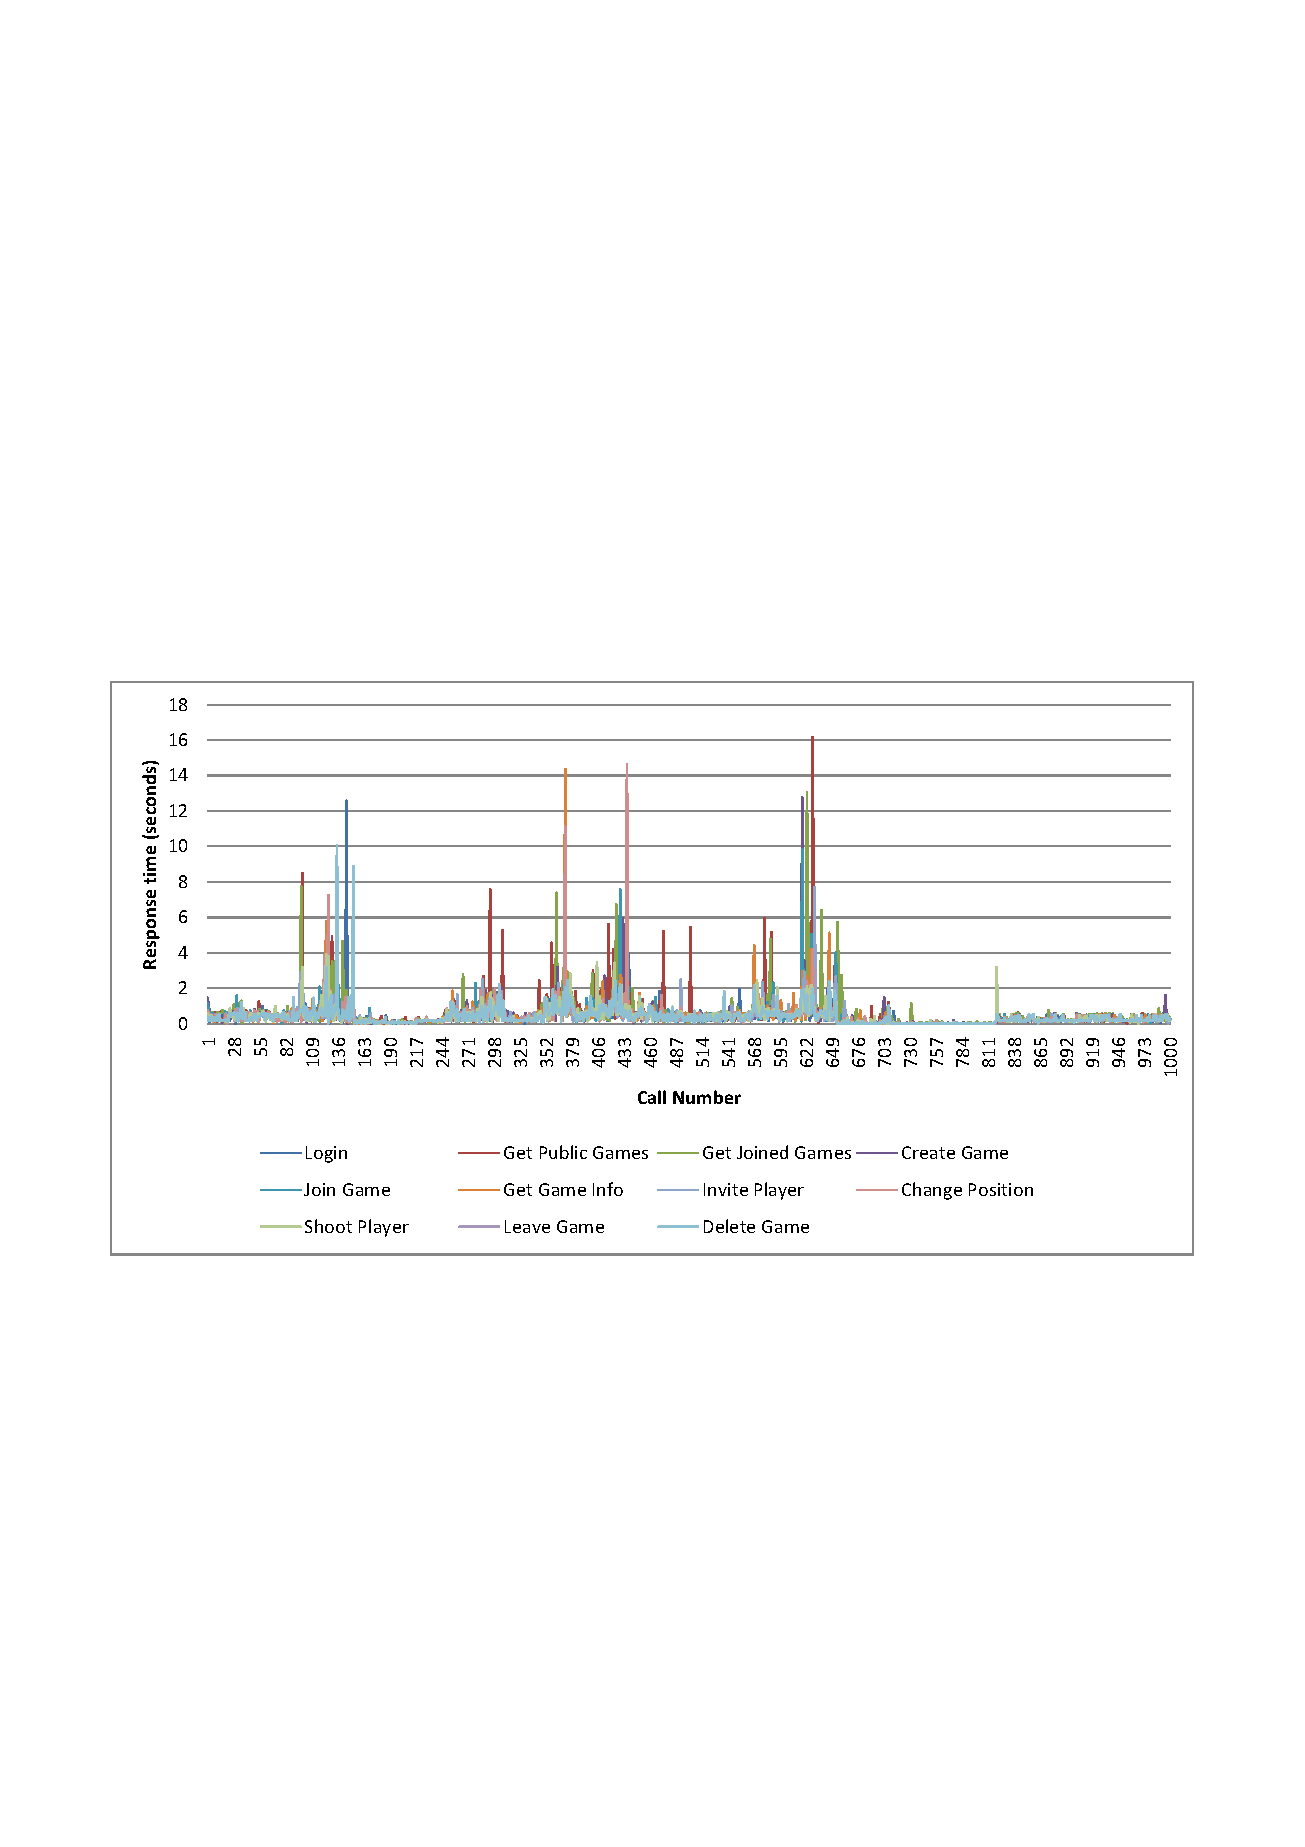
\includegraphics[width=\textwidth, clip=true, trim=0 22em 0 22em]{billeder/loadgraph.pdf}  
  \caption{Graph showing the response time of each API call.}
  \label{fig:loadgraph}
\end{figure}

\renewcommand{\arraystretch}{1.2}
\begin{table}
\caption{Test with no load}
\label{tab:unloadgraph}
\centering
\begin{tabular}{|l|>{\raggedleft\arraybackslash}p{5em}|>{\raggedleft\arraybackslash}p{5em}|>{\raggedleft\arraybackslash}p{5em}|>{\raggedleft\arraybackslash}p{5em}|}
	\hline  & \multicolumn{1}{p{5em}|}{Mean of response time (sec)} & \multicolumn{1}{p{5em}|}{Number over limit} & \multicolumn{1}{p{5em}|}{Number timed out} \\ 
	\hline Login  & 0.0135 & 3 & 0 \\ 
	\hline Get public games  & 0.0118 & 2 & 0 \\ 
	\hline Get joined games  & 0.0565 & 10 & 1 \\ 
	\hline Create game  & 0.0131 & 1 & 0 \\ 
	\hline Join game  & 0.0118 & 2 & 0 \\ 
	\hline Get game info  & 0.0114 & 2 & 0 \\ 
	\hline Invite player  & 0.0100 & 1 & 0 \\ 
	\hline Change position  & 0.0097 & 0 & 1 \\ 
	\hline Shoot player  & 0.0168 & 3 & 0 \\ 
	\hline Leave game  & 0.0067 & 1 & 1 \\ 
	\hline Delete game  & 0.0102 & 0 & 0 \\ 
	\hline 
\end{tabular} 
\end{table}

\begin{table}
\caption{Test with load}
\label{tab:loadgraph}
\centering
\begin{tabular}{|l|>{\raggedleft\arraybackslash}p{5em}|>{\raggedleft\arraybackslash}p{5em}|>{\raggedleft\arraybackslash}p{5em}|>{\raggedleft\arraybackslash}p{5em}|}
	\hline  & \multicolumn{1}{p{5em}|}{Mean of response time(sec)} & \multicolumn{1}{p{5em}|}{Number over limit} & \multicolumn{1}{p{5em}|}{Number timed out} \\ 
	\hline Login  & 0.3676 & 262 & 1 \\ 
	\hline Get public games  & 0.4825 & 328 & 0 \\ 
	\hline Get joined games  & 0.4959 & 353 & 0 \\ 
	\hline Create game  & 0.4143 & 306 & 0 \\ 
	\hline Join game  & 0.4096 & 289 & 0 \\ 
	\hline Get game info  & 0.4051 & 279 & 0 \\ 
	\hline Invite player  & 0.3752 & 273 & 0 \\ 
	\hline Change position  & 0.4050 & 276 & 0 \\ 
	\hline Shoot  & 0.3806 & 259 & 0 \\ 
	\hline Leave game  & 0.3814 & 253 & 0 \\ 	
	\hline Delete game  & 0.3721 & 299 & 0 \\ 
	\hline 
\end{tabular} 
\end{table}
\renewcommand{\arraystretch}{1}